\chapter{Background}\label{chapter:background}
\addcontentsline{toc}{chapter}{Background}

\section{Proteine}\label{sec:proteine}
Le proteine sono considerate il più importante strumento molecolare con le quali è possibile esprimere l'informazione genetica. 

Come riporta \cite{Principi}, le proteine di qualsiasi organismo, dai batterei più semplici agli essere umani, sono formate sempre dalla stessa serie di venti amminoacidi. Poiché ogni amminoacido ha una catena laterale con specifiche proprietà chimiche, questo gruppo di 20 precursori può essere considerato come una forma di alfabeto con cui è scritto il linguaggio della struttura delle proteine. 

Gli amminoacidi, in modo retorico, possono essere considerati dei mattoncini che costruiscono le proteine e giocando con questi mattoncini possiamo costruire diverse tipologie di proteine. 
Come riporta \cite{Principi}, le proteine sono polimeri di amminoacidi in cui ogni residuo amminoacidico  è unito a quello vicino da uno specifico legame covalente. Il legame covalente in questione è il legame peptidico o giunto peptidico che unisce il gruppo (-NH2) di un amminoacido con il gruppo (-COOH) di un altro amminoacido. Negli organismi viventi le proteine svolgono innumerevoli funzioni, tra cui la catalisi delle reazioni metaboliche, funzione di sintesi come replicazione del DNA, la risposta a stimoli e il trasporto di molecole da un luogo ad un altro. Le proteine in generale si differiscono nella sequenza degli amminoacidi, che viene conservata nei geni e che si traduce in un particolare ripiegamento della stessa e una struttura tridimensionale specifica che caratterizza la sua attività.

\subsection{Amminoacidi}\label{subsec:amminoacido}
Tutti gli amminoacidi presenti nelle proteine sono $\alpha$-amminoacidi. Essi sono composti da un gruppo carbosillico e un gruppo amminico legati allo stesso atomo di carbonio, denominato carbonio $\alpha$, e si distinguono l'uno dall'altro mediante il gruppo R, che si differenzia non solo per la struttura, ma anche per proprietà chimico-fisiche, Fig.\ref{fig:Amminoacido}. 
\begin{figure}
	\centering
	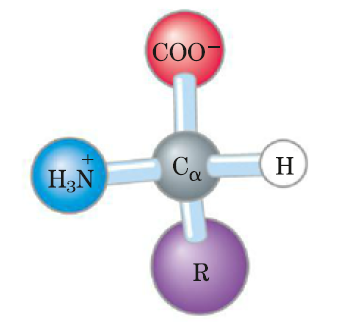
\includegraphics[width=0.3\textwidth]{Immagini/StrutturaAmminoacido.png}
	\caption{La struttura è comune a tutti gli amminoacidi. Il gruppo R è legato al carbonio $\alpha$ ed è diverso per ogni amminoacido. Solo nel caso della glicina il gruppo R è un atomo di idrogeno}
	\label{fig:Amminoacido}
\end{figure}

Nei comuni amminoacidi, il carbonio $\alpha$ è legato a quattro gruppi differenti: il gruppo carbosillico; il gruppo amminico; il gruppo R; un'atomo di idrogeno. Il carbonio $\alpha$ è detto centro chirale, ovvero ha quattro sostituenti diversi ed è asimmetrico. 

\subsubsection{Classificazione degli amminoacidi}\label{subsubsec:classiamminoacido}
\begin{table}[h]
	\centering
	\fontfamily{ptm}\selectfont
	\label{tab:gruppoamminico}
	\begin{tabularx}{1\textwidth}{|l|l|l|l|l|l|l|l|l|}
		\hline
		\parbox{1.8cm}{\textbf{\small Ammino-\\acido}} & \parbox{1.4cm}{\textbf{\small Simbolo}} & \parbox{0.1cm}{$\mathbf{\small{M_r}}$} & \parbox{0.1cm}{$\mathbf{\small{pK_1}}$} & \parbox{0.1cm}{$\mathbf{\small{pK_2}}$} & \parbox{0.1cm}{$\mathbf{\small{pK_r}}$} & \parbox{0.1cm}{\textbf{pl}} & \parbox{1cm}{\textbf{\small Indice idropatico}} & \parbox{1.35cm}{\textbf{\small Presenza nelle proteine \%}}  \\ \hline
		\multicolumn{9}{!{\vrule width 1pt}>{\columncolor{gray!25}}c!{\vrule width 1pt}}{\textbf{Gruppi R alifatici, non polari}} \\ \hline
		\parbox{0.4cm}{\small Glicina}& Gly & 75 & 2.34 & 9.60 & & 5.97 & -0.4 & 7.2\\ \hline
		\parbox{0.4cm}{\small Alanina} & Ala & 89 & 2.34 & 9.69 & & 6.01 & 1.8 & 7.8 \\ \hline
		\parbox{0.4cm}{\small Prolina} & Pro & 115 & 1.99 & 10.96 & & 6.48 & -1.6 & 5.2\\ \hline
		\parbox{0.4cm}{\small Valina} & Val & 117 & 2.32 & 9.62 & & 5.97 & 4.2 & 6.6 \\ \hline
		\parbox{0.4cm}{\small Leucina} & Leu & 131 & 2.36 & 9.60 & & 5.98 & 3.8 & 9.1\\ \hline
		\parbox{0.4cm}{\small Isoleucina} & Ile & 131 & 2.36 & 9.68 & & 6.02 & 4.5 & 5.3 \\ \hline
		\parbox{0.4cm}{\small Metionina} & Met & 149 & 2.28 & 9.21 & & 5.74 & 1.9 & 2.3 \\ \hline
		\multicolumn{9}{!{\vrule width 1pt}>{\columncolor{gray!25}}c!{\vrule width 1pt}}{\textbf{Gruppi R aromatici}} \\ \hline
		\parbox{0.4cm}{\small Fenilalanina} & Phe & 165 & 1.83 & 9.13 & & 5.48 & 2.8 & 3.9\\ \hline
		\parbox{0.4cm}{\small Tirosina} & Tyr & 181 & 2.20 & 9.11 & 10.07 &5.66 & -1.3 & 3.2\\ \hline
		\parbox{0.4cm}{\small Triptofano} & Trp & 204 & 2.38 & 9.39 & & 5.89 & -0.9 & 1.4 \\ \hline
		\multicolumn{9}{!{\vrule width 1pt}>{\columncolor{gray!25}}c!{\vrule width 1pt}}{\textbf{Gruppi R polari, non carichi}} \\ \hline
		\parbox{0.4cm}{\small Serina} & Ser & 105 & 2.21 & 9.15 & & 5.68 & -0.8 & 6.8 \\ \hline
		\parbox{0.4cm}{\small Treonina} & Thr & 119 & 2.11 & 9.62 & & 5.87 & -0.7 & 5.9 \\ \hline
		\parbox{0.4cm}{\small Cisteina} & Cys & 121 & 1.96 & 10.28 & 8.18 & 5.07 & 2.5 & 1.9 \\ \hline
		\parbox{0.4cm}{\small Asparagina} & Asn & 132 & 2.02 & 8.80 & & 5.41 & -3.5 & 4.3 \\ \hline
		\parbox{0.4cm}{\small Glutammina} & Gln & 146 & 2.17 & 9.13 & & 5.65 & -3.5 & 4.2 \\ \hline
		\multicolumn{9}{!{\vrule width 1pt}>{\columncolor{gray!25}}c!{\vrule width 1pt}}{\textbf{Gruppi R carichi positivamente}} \\ \hline
		\parbox{0.4cm}{\small Lisina} & Lys & 146 & 2.18 & 8.95 & 10.53 & 9.74 & -3.9 & 5.9\\ \hline
		\parbox{0.4cm}{\small Istidina} & His & 155 & 1.82 & 9.17 & 6.00 & 7.59 & -3.2 & 2.3\\ \hline
		\parbox{0.4cm}{\small Arginina}& Arg & 174 & 2.17 & 9.04 & 12.48 & 10.76 & -4.5 & 5.1\\ \hline
		\multicolumn{9}{!{\vrule width 1pt}>{\columncolor{gray!25}}c!{\vrule width 1pt}}{\textbf{Gruppi R carichi negativamente}} \\ \hline
		\parbox{0.4cm}{\small Aspartato} & Asp & 133 & 1.88 & 9.60 & 3.65 & 2.77 & -3.5 & 5.3 \\ \hline
		\parbox{0.4cm}{\small Glutammato} & Glu & 147 & 2.19 & 9.67 & 4.25 & 3.22 & -3.5 & 6.3 \\ \hline
	\end{tabularx}
	\normalfont
	\caption{Proprietà e nomenclatura degli amminoacidi comuni presenti nelle proteine.}
	\smallskip
	\begin{tablenotes}
		\item[\dag] \textbf{Indice idropatico} è un valore che combina idrofobicità e idrofilicità dei gruppi R e si riferisce all'energia libera di trasferimento ($\delta G$) della catena laterale dell'amminoacido da un solvente idrofobico all'acqua. Il trasferimento è favorito ($\delta G < 0$, valore dell'indice negativo) per le catene laterali degli amminoacidi carichi o polari; ed è sfavorito ($\delta G > 0$, valore dell'indice positivo) per le catene laterali degli amminoacidi non polari o idrofobici.
		\item[\ddag] \textbf{Presenza nelle proteine \%} rappresenta la presenza media in più di 1150 proteine.
	\end{tablenotes}
\end{table}

Gli amminoacidi possono essere classificati sulla base della caratteristiche chimico-fisiche del gruppo R legato al carbonio $\alpha$:
\vspace{10pt}
\begin{itemize}
	\item Gruppi R alifatici, non polari: in questa classe gli amminoacidi non sono polari e quindi idrofobici; le catene laterali tendono a interagire all'interno della proteina tramite interazioni idrofobiche;
	\vspace{5pt}
	\item Gruppi R aromatici: in questa classe gli amminoacidi sono tutti non polari (idrofobici) e tutti possono intervenire nelle interazioni idrofobiche;
	\vspace{5pt}
	\item Gruppi R polari, non carichi: in questa classe gli amminoacidi sono più solubili in acqua (o più idrofilici), rispetto ai non polari, perché contengono gruppi funzionali che creano legami idrogeno;
	\vspace{5pt}
	\item Gruppi R carichi positivamente: in questa classe gli amminoacidi, sono quelli più idrofilici poichè contengono una carica netta positiva;
	\vspace{5pt}
	\item Gruppi R carichi negativamente: in questa classe gli amminoacidi, sono quelli più idrofilici poichè contengono una carica netta negativa e sono caratterizzati dall'avere un secondo gruppo carbosillico.
	\vspace{5pt}
\end{itemize}

\subsection{Polimeri degli amminoacidi}\label{subsec:polimeri}
Le proteine differiscono nel numero di amminoacidi che li compongono. Due molecole di amminoacidi come detto in precedenza possono unirsi covalentemente mediante un legame ammidico, chiamato appunto legame peptidico, formando un dipeptide. Come dice \cite{Principi}, questo tipo di legame si genera per eliminazione di una molecola d'acqua dal gruppo $\alpha$-carbosillico di un amminoacido e dal gruppo $\alpha$-amminico dell'altro (Fig. \ref{fig:legamepeptidico}). 

\begin{figure}
	\centering
	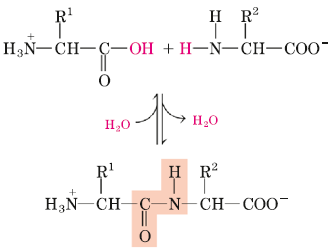
\includegraphics[width=0.5\textwidth]{Immagini/LegamePeptidico.png}
	\caption{Formazione di un legame peptidico per condensazione, li gruppo $\alpha$-amminico di un amminoacido (con ilgruppo R2) agisce da nucleofilo e reagisce con Il gruppo ossidrilico del carbossile di un altro amminoacido (con Il gruppo R1), formando un legame peptidico (ombreggiato in rosa).}
	\label{fig:legamepeptidico}
\end{figure}

Oligopeptidi e Polipeptidi differiscono per il numero di amminoacidi costituenti. I polipeptidi o proteine sono delle macromolecole a struttura complessa costituite da un numero di unità monometriche convenzionalmente  superiore a 50. Alcune proteine sono costituite da una singola catena polipetidica, mentre altre hanno più polipetidi associati in modo non covalente e sono chiamate proteine multisubunità. All'interno delle proteine multisubunità, se almeno due dei polipeptidi presenti sono uguali, allora la proteina viene detta oligomerica, e le subunità identiche sono dette protomeri. Come riporta \cite{Principi}, la composizione amminoacidica delle proteine è molto variabile. Infatti i 20 amminoacidi comuni non sono quasi mai distribuiti in egual proporzione nella proteina.

Una volta espresse, alcune proteine possono subire delle modifiche chimico-strutturali essenziali per la loro funzione. Tra queste ricordiamo la glicosilazione, una modifica post-tradizionale tale per cui alcuni residui aminoacidici sono non-covalentemente legati a zuccheri, molecole formate da un anello a cinque o sei atomi di carbonio legati a gruppi ossidrilici
 
\subsection{Struttura delle proteine}\label{subsec:strutturaproteine}
Le caratteristiche strutturali conferiscono alla proteina stessa la sua funzione, ma la struttura di una proteina di grandi dimensioni è complessa e può essere descritta secondo vari livelli di complessità. In generale vengono descritti quattro livelli di struttura delle proteine, come si può vedere nella Fig. \ref{fig:strutturagerarchica}. 

\begin{figure}
	\centering
	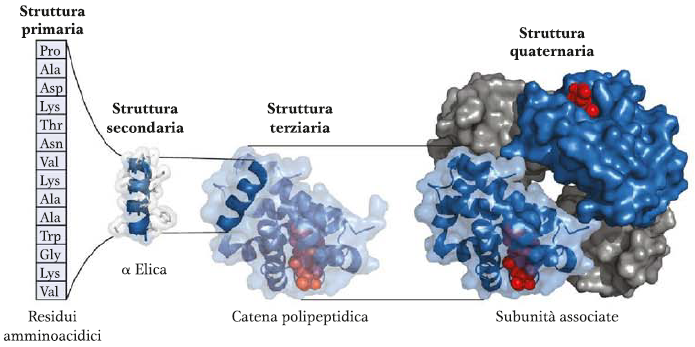
\includegraphics[width=0.8\textwidth]{Immagini/StrutturaGerarchica.png}
	\caption{Livelli di struttura delle proteine. La struttura primaria è una sequenza di amminoacidi unita da legame peptidico. I polipeptidi risultanti possono disporsi in una struttura regolare ricorrente che viene definita struttura secondaria, come l'$\alpha$ elica. Essa costituisce una delle parti della struttura terziaria, che può essere a sua volta una delle subunità della struttura quaternaria.}
	\label{fig:strutturagerarchica}
\end{figure}

La struttura primaria è costituita da tutti i legami covalenti che legano tra loro i vari amminoacidi della catena polipeptidica. La struttura secondaria contiene organizzazioni particolari e stabili di brevi sequenze di amminoacidi, che danno il via a profili strutturali ricorrenti. La struttura terziaria descrive l'aspetto tridimensionale del polipeptidico, mentre se sono presenti più unità allora è presente anche la struttura quaternaria. In particolar modo la struttura primaria di una proteina determina la disposizione degli atomi nello spazio tridimensionale che ne caratterizzano la funzione. 

Come riporta \cite{Principi}, la disposizione spaziale degli atomi di una proteina, o di una porzione di proteina è detta conformazione. Le conformazioni possibili di una proteina, o di una parte di essa, corrispondono a tutte le strutture che la proteina può assumere senza rottura di legami covalenti. 
I legami covalenti perciò hanno un ruolo importante nel determinare la conformazione di un polipeptide. Gli atomi di carbonio $\alpha$ di residui amminoacidici adiacenti sono separati da tre legami covalenti che si susseguono in questo modo: $C_\alpha$---C---N---$C_\alpha$. Facendo analisi su questi atomi del gruppo peptidico, si evince che i legami C---N, a causa del loro parziale carattere di doppio legame non può ruotare liberamente; è invece concessa la rotazione tra i legami N---$C_\alpha$ e $C_\alpha$---C. Lo scheletro della catena polipeptidica può quindi essere considerato una serie di piani rigidi, in cui i piani consecutivi hanno come punto di rotazione in comune $C_\alpha$ (Fig. \ref{fig:gruppopeptidico}). La rigidità del legame limita considerevolmente la possibilità di movimento e di conseguenza il numero delle conformazioni che possono essere assunte. La conformazione è poi specificata dai tre angoli diedrici (o angoli torsionali) chiamati $\phi$ (phi), $\psi$ (psi) e $\omega$ (omega). 

La struttura secondaria si riferisce ad un segmento polipeptidico della proteina e descrive l'organizzazione spaziale della catena principale senza considera le catene laterali. Le strutture secondarie regolari più comuni sono l'$\alpha$ elica, la conformazione $\beta$ foglietto e il ripiegamento $\beta$. La struttura terziaria corrisponde alla struttura tridimensionale completa di una catena polipeptidica e in base ad essa si possono distinguere due classi di proteine: le fibrose e le globulari.La struttura quaternaria deriva dalle interazioni tra le subunità che costituiscono una proteina multimerica. 

\begin{figure}
	\centering
	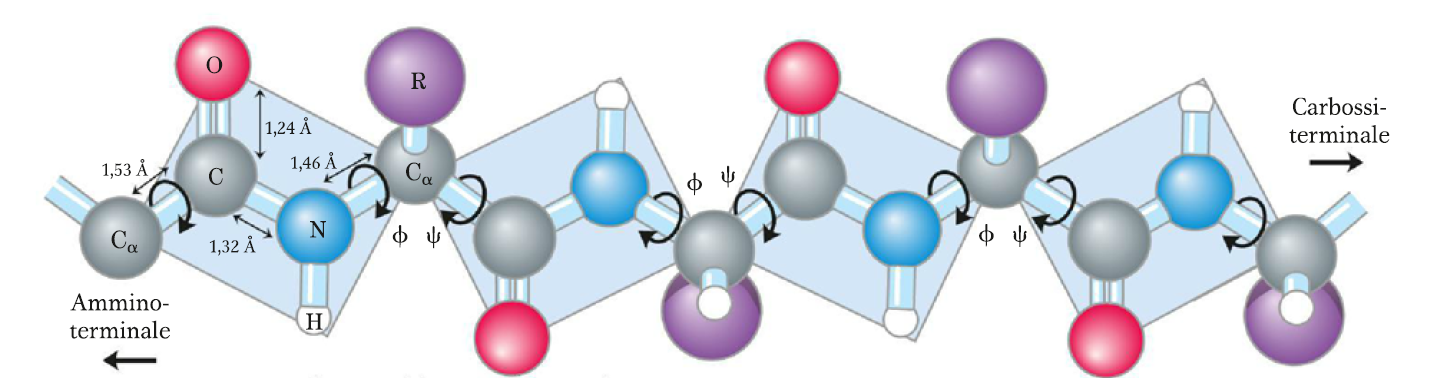
\includegraphics[width=0.8\textwidth]{Immagini/Gruppopeptidicoplanare.png}
	\caption{Tre legami separano due atomi di carbonio $\alpha$ in successione in una catena polipeptidica. I legaml N---$C_\alpha$ e $C_\alpha$---C possono ruotare, descrivendo due angoli diedrici chiamati rispettivamente $\phi$ e $\psi$. Il legame C---N non è libero di ruotare. La rotazione degll altri legami singoli dello scheletro peptidico è resa difficoltosa dalle dimensioni e dalle cariche del gruppi R.}
	\label{fig:gruppopeptidico}
\end{figure}


\subsection{Classificazione delle proteine}\label{subsec:classificazioneproteine}
Le proteine hanno molteplici funzioni, sono coinvolte nel movimento, nella trasmissione dei segnali (ormoni), proteggono l'organismo (anticorpi), mantengono le sostanze, le trasportano, fungono da enzima, hanno funzione recettoriale e anche strutturale.E' possibile classificare le proteine sulla base della loro funzione come segue:
\vspace{10pt}
\begin{itemize}
	\item proteine di trasporto: facilitano il trasporto passivo (per diffusione) o attivo (attraverso legame chimico e consumo di energia) di sostanze attraverso le membrane biologiche e nei vari tessuti. Ne è un esempio l'emoglobina, che trasporta ossigeno dai polmoni ai tessuti, e la mioglobina che permette di veicolare l'ossigeno ai mitocondri presenti nelle cellule del tessuto muscolare;
	\vspace{5pt}
	\item proteine implicate nella segnalazione cellulare: permettono la trasmissione di segnali chimici o elettrici essenziali per la vita cellulare. Appartengono a questa categoria anche gli anticorpi prodotti  dai linfociti B attivati in risposta agli antigeni, come batteri, virus e altre sostanze riconosciute come microorganismi e agenti estranei pericolosi;
	\vspace{5pt}
	\item enzimi: gli enzimi sono le proteine responsabili della catalisi delle reazioni chimiche all'interno del nostro organismo. Di fatto accelerano una reazione chimica specifica senza essere consumati e senza entrare nei prodotti finali della reazione;
	\vspace{5pt}
	\item proteine strutturali: tipicamente formano delle strutture di sostegno, si tratta infatti di molecole caratterizzate da durezza e resistenza, un esempio può essere l'$\alpha$-cheratina che forma le strutture interne dell'organismo.
	\vspace{5pt}
\end{itemize}

\subsection{Principio di Ramachandran}\label{subsec:ramachandranPrinciple}
Il principio di Ramachandran ha stabilito che solo alcune conformazioni di angoli di torsione sono stabili e presenti naturalmente nelle proteine. Queste conformazioni stabili sono descritte come regioni favorevoli o regioni accettabili nel grafico di Ramachandran. Le conformazioni non favorevoli o non accettabili sono associate con strutture instabili o anomale.

Il principio di Ramachandran è spesso molto utile per saggiare la qualità e l'attendibilità delle strutture tridimensionali delle proteine. 

Le conformazioni dei peptidi sono definite come descritto in precedenza da $\phi$ e $\psi$, che possono assumere qualsiasi valore compreso tra $-180°$ e $+180°$. Non tutte le coppie di angoli torsionali teoricamente possibili sono realmente ottenibili all'interno delle strutture peptidiche in quanto impedite dalla presenza di ingombri sterici fra i gruppi delle catene laterali, basati su calcoli in cui sono utilizzati il raggio di van der Walls e gli angoli di legame. Come si può vedere nella Fig. \ref{fig:graficoRamachandran}, le aree colorate in blu scuro, contengono le conformazioni che non presentano sovrapposizioni steriche, ovvero quando ogni atomo può essere mostrato come una sfera solida, di conseguenza sono zone completamente consentite. Le zone evidenziate con un colore intermedio sono zone in cui è presente un piccolo scontro; quindi, se viene concesso uno scontro di 0.1 nm sono conformazioni concesse. Le zone evidenziate in azzurro sono consentito a patto che sia consentita una leggera flessibilità dell'angolo $\omega$. Le regioni non evidenziate sono zone non consentite. Si può notare la poca simmetria presente nel grafico, a causa della stereochimica dei residui amminoacidici.
\begin{figure}
	\centering
	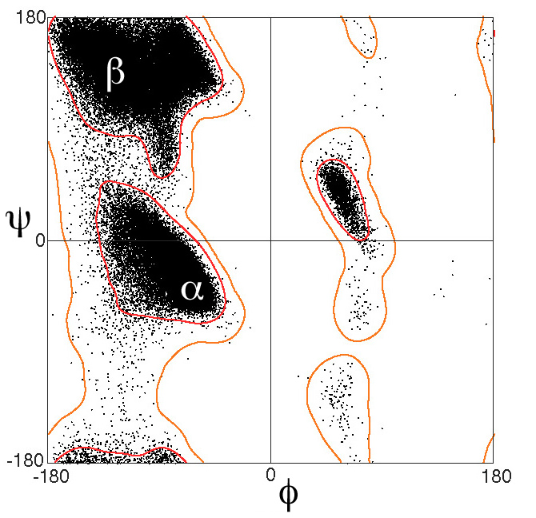
\includegraphics[width=0.6\textwidth]{Immagini/GraficoRamachandran.png}
	\caption{Esempio grafico di Ramachandran}
	\label{fig:graficoRamachandran}
\end{figure}

\section{Hydropathic INTeractions HINT}\label{sec:cap_sec_subsec}

Come riportato da \cite{AgostaCozzini}, la valutazione della stabilità intramolecolare di una proteina gioca un ruolo fondamentale nella comprensione del comportamento e del meccanismo di azione. Piccole alterazioni strutturali possono impattare l'attività biologica e di conseguenza la modulazione farmacologica. 
L'analisi della struttura tridimensionale della proteina e la risultante stabilità permettono di predire un possibile meccanismo di attivazione e rivelano nuove strategie per scoprire nuovi farmaci. Ogni modifica apportata alla struttura di una proteina porta quasi sicuramente ad una variazione del suo meccanismo di azione, e valutare la stabilità di una proteina può essere molto costoso in termini di tempo.
La stabilità delle proteine è influenzata dalle interazioni intramolecolare, ovvero sono forze che permettono di creare e tenere insieme una struttura. Le strutture native delle proteine sono stabili poiché si formano come risultato di un equilibrio tra le varie forze non covalenti a cui sono soggette: i legami idrogeno, i legami ionici, le forze di Wan der Walls e le interazioni idrofobiche. In generale le interazioni chimiche deboli sono attrazzioni tra atomi appartenenti o alla stessa molecola (intramolecolari) o a molecole diverse (intermolecolari). Le interazioni chimiche deboli si formano e si rompono in continuazione alla temperatura fisiologica dell'organismo. a meno che, cumulandosi in gran numero, esse non diano collettivamente stabilità alle strutture che contribuiscono a generare.

La valutazione della stabilità intramolecolare di una proteina è particolarmente complessa e ha portato allo sviluppo e ottimizzazione di metodi computazionali differenti che vanno dalla meccanica classica ai più recenti algoritmi di machine Learning

HINT (Hydrophatic INTeractions) è un programma designato per quantificare le interazioni inter e intramolecolari, come citato in \cite{Kellogg1991} e in \cite{EUGENEKELLOGG2000651}.
In breve, sulla base di valori di LogPo/W (coefficiente di ripartizione ottanolo/acqua di una sostanza, indice della sua polarità/idrofobicità) calcolati per tutti gli amminoacidi del sistema è possibile classificare e quantificare le interazioni calcolati come il prodotto tra la superficie accessibile al solvente e la costante idrofobica di ogni atomo e la loro distanza, come descritto in \cite{ExtensionFragment}. La funzione di energia intramolecolare di HINT può essere calcolata rapidamente dalla struttura in termini di somma di punteggi d'interazione atomo-atomo. Il punteggio intramolecolare viene calcolato come somma delle interazioni idrofobiche e polari tra tutte le coppie di atomi considerando l'area accessibile al solvente. Le interazioni idrofobiche si verificano quando le molecole non polari si avvicinano tra di loro in un solvente polare, come l'acqua. Le molecole non polari tendono a respingersi reciprocamente e ad attirarsi con le molecole del solvente. Il processo anche noto come esclusione dei solventi, porta alla formazioni di molecole non polari all'interno del solvente. Le molecole non polari quindi cercano di organizzarsi in modo tale da minimizzare il contatto con il solvente e massimizzare le interazioni tra di loro. 

Il punteggio energetico di HINT intramolecolare consente quindi di calcolare tutte le interazioni idropatiche (idrofobiche e polari) che si verificano nella molecola e ne consentono di valutare la stabilità termodinamica. Dato il suo livello di sensibilità nell'individuare piccole differenze di energie verrà poi utilizzato per stimare la stabilità della Glicoproteina spike del SARS-CoV-2.

\section{Ricerca Locale}\label{sec:cap_sec_subsec}
La ricerca locale è una tecnica euristica di ottimizzazione e risoluzione dei problemi che mira a trovare una soluzione che sia vicina alla soluzione attuale e la migliore. 
Funziona apportando piccole modifiche alla soluzione corrente e valutando i risultati, con l'obiettivo di trovare una soluzione ottimale in uno spazio di ricerca 
limitato. La ricerca locale viene spesso utilizzata nei problemi di ottimizzazione combinatoria, come il problema del commesso viaggiatore, e nell'apprendimento 
automatico, dove può essere utilizzata per ottimizzare algoritmi complessi come le reti neurali. L'idea chiave alla base della ricerca locale è evitare di rimanere 
bloccati in soluzioni non ottimali apportando una serie di piccole modifiche informate alla soluzione corrente fino a quando non viene trovata una soluzione ottimale.

La ricerca locale è un sottocampo di:
\vspace{10pt}
\begin{itemize}
    \item Metaheuristic: è una procedura o euristica di livello superiore progettata per trovare, generare o selezionare un'euristica che può fornire una soluzione
    sufficientemente buona a un problema di ottimizzazione, in particolari con informazioni incomplete o limitate capacità di calcolo;
    \vspace{5pt}
    \item Stochastic optimization: sono metodi di ottimizzazione che generano e utilizzano variabili casuali; I metodi di ottimizzazione stocastica generalizzano metodi 
    deterministici per problemi deterministici;
    \vspace{5pt}
    \item Mathematical optimization: è la selezione di un elemento migliore rispetto ad un qualche criterio, da un insieme di alternative disponibili; Nell'approccio 
    più generale, un problema di ottimizzazione consiste nel massimizzare o minimizzare una funzione reale scegliendo sistematicamente i valori di input 
    all'interno di un insieme consentito e calcolando il valore della funzione.
\end{itemize}

La maggior parte dei problemi può essere formulata in termini di spazio di ricerca e target in diversi modi. Ad esempio, per il problema del commesso viaggiatore una 
soluzione può essere un percorso che tocca tutte le città e l'obiettivo è trovare il percorso più breve. Ma una soluzione può anche essere un percorso, che può anche 
contenere un ciclo.

Un algoritmo di ricerca locale parte da una soluzione candidata e quindi si sposta iterativamente verso una soluzione vicina; un quartiere è l'insieme di tutte le 
possibili soluzioni che differiscono dalla soluzione attuale per la minima misura possibile. Ciò richiede la definizione di una relazione di vicinato nello spazio 
di ricerca. Ad esempio, l'intorno della copertura del vertice è un'altra copertura del vertice che differisce solo per un nodo. Per la soddisfacibilità booleana, 
i vicini di un'assegnazione booleana sono quelli che hanno una singola variabile in uno stato opposto. Lo stesso problema può avere più quartieri distinti definiti 
su di esso; l'ottimizzazione locale con quartieri che implicano la modifica di fino a k componenti della soluzione viene spesso definita k-opt.

Tipicamente, ogni soluzione candidata ha più di una soluzione vicina; la scelta di quale selezionare viene presa utilizzando solo le informazioni sulle soluzioni 
nelle vicinanze dell'assegnazione corrente, da cui il nome ricerca locale. Quando la scelta della soluzione del vicino è fatta prendendo quella che massimizza 
localmente il criterio, cioè: una ricerca avida, la metaeuristica prende il nome di hill climbing. Quando non sono presenti vicini in miglioramento, 
la ricerca locale è bloccata in un punto localmente ottimale. Questo problema di ottimo locale può essere risolto utilizzando i riavvii (ricerca locale ripetuta 
con diverse condizioni iniziali), la randomizzazione o schemi più complessi basati su iterazioni, come la ricerca locale iterata, sulla memoria, come 
l'ottimizzazione della ricerca reattiva, su modifiche stocastiche senza memoria, come la simulated annealing.

La ricerca locale non fornisce una garanzia che una determinata soluzione sia ottimale. La ricerca può terminare dopo un determinato periodo di tempo o quando la 
migliore soluzione trovata fino a quel momento non è migliorata in un determinato numero di passaggi. La ricerca locale è un algoritmo anytime: può restituire 
una soluzione valida anche se viene interrotta in qualsiasi momento dopo aver trovato la prima soluzione valida. La ricerca locale è in genere un'approssimazione 
o un algoritmo incompleto, poiché la ricerca potrebbe interrompersi anche se la migliore soluzione corrente trovata non è ottimale. Ciò può accadere anche se 
la terminazione avviene perché la migliore soluzione attuale non può essere migliorata, poiché la soluzione ottima può trovarsi lontano dall'intorno delle 
soluzioni attraversate dall'algoritmo.

Schuurman \& Southey propongono tre misure di efficacia per la ricerca locale (profondità, mobilità e copertura):
\vspace{10pt}
\begin{itemize}
    \item Profondità: il costo dell'attuale (migliore) soluzione;
    \vspace{5pt}
    \item Mobilità: la capacità di spostarsi rapidamente in diverse aree dello spazio di ricerca (mantenendo bassi i costi);
    \vspace{5pt}
    \item Copertura: quanto sistematicamente la ricerca copre lo spazio di ricerca, la distanza massima tra qualsiasi incarico inesplorato e tutti gli incarichi
    visitati.
\end{itemize}

Ipotizzano che gli algoritmi di ricerca locale funzionino bene, non perché abbiano una certa comprensione dello spazio di ricerca, ma perché si spostano 
rapidamente in regioni promettenti ed esplorano lo spazio di ricerca a basse profondità nel modo più rapido, ampio e sistematico possibile.

\subsection{Tipologie di ricerca locale}\label{subsec:es_subsec}
La ricerca locale si basa sul presupposto che il miglioramento di una soluzione che si trovi nelle immediate vicinanze di quest'ultima (vicinato).
Data una qualsiasi soluzione euristica (nodo corrente) la ricerca locale verifica l'esistenza di soluzioni migliori nell'insieme delle soluzioni più vicine 
(nodi vicini). Ad esempio, un algoritmo di ricerca locale può essere utilizzato per risolvere il problema del commesso viaggiatore. 
Le tecniche di ricerca locale consentono di raggiungere risultati sia nella ricerca delle soluzioni a un problema (problem solving) e sia 
nell'ottimizzazione. Appartengono alla categoria degli algoritmi di ricerca locale i seguenti algoritmi:
\begin{itemize}
    \item Ricerca hill climbing: L'algoritmo di ricerca hill climbing è una tecnica di ricerca locale in cui il nodo corrente è sostituito con il nodo migliore;
    \vspace{5pt}
    \item Simulated annealing: L'algoritmo di Simulated annealing o Annealing simulato (SA) è un algoritmo probabilistico-metaeuristico di ottimizzazione 
    della ricerca in uno spazio di ricerca di grandi dimensioni. Il suo nome prende spunto dal processo metallurgico che consente di riaggregare la materia fusa 
    dei metalli in base a determinate caratteristiche comuni. Nell'algoritmo di simulated annealing un processo di selezione consente l'eventuale sostituzione 
    della soluzione del nodo corrente con quella di un nodo selezionato casualmente da una lista di soluzioni candidate;
    \vspace{5pt}
    \item Beam Search. La beam search è una ricerca locale basata su tecniche euristiche. La beam search ( ricerca di fascio ) esplora un fascio limitato di 
    nodi promettenti (soluzioni parziali) dello spazio di ricerca e li analizza con una ricerca locale. Utilizzando le tecniche euristiche l'algoritmo beam search 
    consente di riconoscere quando una soluzione parziale è anche una soluzione completa.
\end{itemize}



\subsection{Euristiche}\label{subsec:es_subsec}
Un algoritmo di tipo Ricerca Locale appartengono alla classe delle euristiche di miglioramento. Sono euristici quegli algoritmi che non garantiscono di fornire 
la soluzione ottima. Ovvero, data una soluzione iniziale ammissibile s, essa è migliorata attraverso successive trasformazioni di s.

Le euristiche sono quindi strategie che aiutano a trovare una soluzione ottimale in una ricerca locale. Ecco alcune delle eurisiche più comuni utilizzate nella 
ricerca locale:
\vspace{10pt}
\begin{itemize}
    \item First-Improvement: Questa euristica cerca sempre la prima soluzione migliore rispetto alla soluzione corrente. Il vantaggio di questa euristica è 
    che è molto veloce, poiché interrompe la ricerca non appena viene trovata una soluzione migliore. Tuttavia, il suo limite è che potrebbe non essere in 
    grado di trovare la soluzione ottimale, poiché potrebbe fermarsi presto;
    \vspace{5pt}
    \item Best-Improvement: Questa euristica cerca sempre la migliore soluzione possibile rispetto alla soluzione corrente. Il vantaggio di questa euristica 
    è che è molto precisa, poiché cerca sempre la soluzione migliore. Tuttavia, il suo limite è che potrebbe essere molto lenta, poiché deve valutare 
    tutte le soluzioni possibili prima di scegliere la migliore;
    \vspace{5pt}
    \item Stochastic Hill Climbing: Questa euristica cerca una soluzione migliore casualmente. Il vantaggio di questa euristica è che è molto flessibile, 
    poiché cerca soluzioni in modo casuale. Tuttavia, il suo limite è che potrebbe essere impreciso, poiché potrebbe scegliere soluzioni subottimali;
    \vspace{5pt}
    \item Simulated Annealing: Questa euristica cerca una soluzione migliore basata sulla probabilità. Il vantaggio di questa euristica è che è molto 
    precisa, poiché cerca soluzioni basate sulla probabilità. Tuttavia, il suo limite è che potrebbe essere molto lenta, poiché deve valutare molte 
    soluzioni prima di scegliere la soluzione migliore;
    \vspace{5pt}
    \item Variable Neighborhood Search: Questa euristica cerca soluzioni migliori cambiando continuamente il vicinato della soluzione corrente. Il vantaggio 
    di questa euristica è che è molto flessibile, poiché cerca soluzioni in molti vicinati diversi. Tuttavia, il suo limite è che potrebbe essere molto lenta, 
    poiché deve valutare molte soluzioni prima di scegliere la soluzione migliore;
    \vspace{5pt}
    \item Greedy Algorithm: Questa euristica seleziona sempre la soluzione che sembra essere la migliore in un determinato momento. Il vantaggio di questa 
    euristica è che è molto veloce, poiché seleziona sempre la soluzione migliore. Tuttavia, il suo limite è che potrebbe non essere in grado di trovare la 
    soluzione ottimale, poiché seleziona sempre la soluzione migliore in un dato momento, senza preoccuparsi delle conseguenze future. Pertanto, 
    è importante utilizzare questo algoritmo con cautela e verificare che la soluzione ottenuta soddisfi i requisiti del problema.
\end{itemize}

\section{Shortest Path}\label{sec:cap_sec_subsec}
Lo shortest path è un importante concetto nell'ambito dell'informatica cosi come nell'ingegneria e nella matematica applicata. Essa si riferisce al percorso più
breve tra due punti in un grafo, ovvero insieme di nodi collegati da archi. 

Esso è molto importante per esempio nel campo della robotica, viene utilizzato per pianificare il percorso del robot, consentendogli di evitare ostacoli e
raggiungere il suo obiettivo in modo efficiente. Possiamo trovare lo stesso concetto applicato nelle reti di telecomunicazioni, poiché viene utilizzato per instradare
il traffico tra due nodi garantendo una comunicazione efficiente e affidabile. Viene anche usato in algoritmi di routing per cercare di minimizzare il tempo di ritardo.
Chiaramente esso si adatta bene nel campo della logistica dove è necessario ottimizzare il trasporto delle merci o delle persone. Infine, trova applicazione anche nel
campo della progettazione di circuiti elettronici.

\subsection{Algoritmo A*}\label{subsec:es_subsec}
L'algoritmo A* è spesso utilizzato nella risoluzione del problema dello shortest path, ovvero per trovare il percorso più breve tra due nodi in un grafo pesato. 
L'algoritmo A* utilizza una funzione di stima euristica per guidare la ricerca verso il percorso più breve, permettendo di ottenere un'efficace combinazione di completezza e velocità nell'individuare la soluzione.

Nella versione dello shortest path risolto con l'algoritmo A*, ogni nodo del grafo viene valutato in base alla sua distanza dal nodo di partenza, la stima della distanza dal nodo di arrivo e il costo totale del percorso, ovvero la somma della distanza dal nodo di partenza e della stima della distanza dal nodo di arrivo. In questo modo, l'algoritmo A* tiene traccia del percorso più breve scoperto fino a quel momento e lo utilizza per determinare quale nodo espandere successivamente.

L'algoritmo A* può essere ulteriormente ottimizzato attraverso l'utilizzo di tecniche come la memorizzazione della distanza minima calcolata per ogni nodo, in modo da ridurre il numero di espansioni necessarie. Inoltre, l'algoritmo A* può essere utilizzato con successo in grafi di grandi dimensioni, grazie alla sua capacità di selezionare le espansioni più promettenti e di escludere le aree meno promettenti del grafo.

\subsection{Esempio}\label{subsec:es_subsec}
In questo esempio, la funzione A\_star prende in input la cella di partenza 'start', la cella di arrivo 'goal' e una rappresentazione del labirinto come 'graph'. La funzione A\_star esplora le celle adiacenti alla cella corrente, calcola il costo del percorso per ogni cella e aggiunge le celle alla coda di priorità. La coda di priorità è ordinata in base al costo totale, che è la somma del costo del percorso e della stima euristica. La funzione A\_star restituisce il percorso più breve dal punto di partenza al punto di arrivo.

\begin{minipage}{\textwidth}
	\begin{lstlisting}[caption={Algoritmo A*}]
		# Definizione della funzione di costo
		def cost(current, next):
			if current[0] == next[0] or current[1] == next[1]:
				return 1
			else:
				return math.sqrt(2)
		
		# Definizione della funzione euristica
		def heuristic(current, goal):
			return math.sqrt((current[0]-goal[0])**2 + (current[1]-goal[1])**2)
		
		# Definizione dell'algoritmo A*
		def A_star(start, goal, graph):
			queue = []
			heapq.heappush(queue, (0, start, []))
			visited = set()
			
			while queue:
				_, current, path = heapq.heappop(queue)
				if current == goal:
				return path + [current]
				if current in visited:
					continue
				visited.add(current)
				for neighbor in graph[current]:
					if neighbor in visited:
						continue
					new_cost = cost(current, neighbor)
					total_cost = new_cost + heuristic(neighbor, goal)
					heapq.heappush(queue, (total_cost, neighbor, path + [current]))
			return None
	\end{lstlisting}
\end{minipage}

\section{Algebra e Geometria}\label{sec:algebra}
L'algebra e la geometria sono due aree fondamentali della matematica che sono strettamente correlate e si influenzano a vicenda. La geometria si occupa dello studio delle figure geometriche nello spazio, come punti, linee, piani, poligoni, solidi e curve. 

L'algebra, come accennato in precedenza, si occupa dello studio delle proprietà delle operazioni aritmetiche e delle relazioni tra le variabili. L'algebra fornisce uno strumento matematico molto potente per la risoluzione di problemi e l'espressione di relazioni matematiche in modo astratto.

L'algebra e la geometria sono strettamente correlate, poiché l'algebra può essere utilizzata per risolvere problemi geometrici, come ad esempio la determinazione di equazioni di rette e di superfici, la risoluzione di equazioni di secondo grado che descrivono curve, e la risoluzione di problemi di trigonometria.

D'altra parte, la geometria può essere utilizzata per visualizzare le relazioni algebriche, ad esempio rappresentando graficamente le funzioni algebriche o le equazioni differenziali.

\subsection{Spazio vettoriale}\label{subsec:spazi_vettoriali}
Gli spazi vettoriali sono una struttura algebrica complessa, composta da: un campo, in cui gli elementi sono detti scalari; un insieme, i cui elementi sono detti vettori; due operazioni binarie, la somma e la moltiplicazione scalare con determinate proprietà. 

Per ogni numero naturale $n \ge 1$ consideriamo l'insieme $\mathbf{R}^n$ delle n-uple ordinate di numeri reali: 

	$$\mathbf{R}^n = \{v = (x_1, .., x_n)| x_i \in \mathbf{R}\}$$.

Viene chiamato $\mathbf{R}^n$ lo spazio n-dimensionale e i suoi elementi vettori o punti, come descritto in \cite{Algebra}. 
\begin{figure}
	\centering
	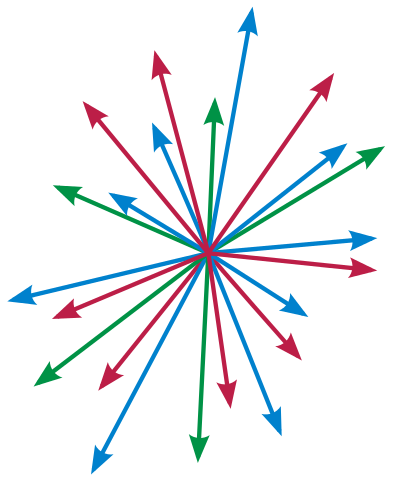
\includegraphics[width=0.3\textwidth]{Immagini/SpazioVettoriale.png}
	\caption{Uno spazio vettoriale è una collezione di oggetti, chiamati "vettori", che possono essere sommati e riscalati.}
	\label{fig:vettori}
\end{figure}
Presi due vettori $$v = (x_1, .., x_n) e w = (y_1, .., y_n)$$ si possono sommare componente per componente per ottenere un nuovo vettore: 

	$$v + w = (x_1 + y_1, .., x_n + y_n)$$.

Un numero $c \in \mathbf{R}$ si può moltiplicare con un vettore $v = (x_1, .., x_n)$ in modo da ottenere un nuovo vettore:

	$$cv = (cx_1, .., cx_n)$$.

Le operazioni di somma e moltiplicazione per scalare sono anche chiamate operazioni di spazio vettoriale. 

Per la somma di vettori $v, w, u \in \mathbf{R}$ vengono verificate le seguenti proprietà:
\vspace{10pt}
\begin{itemize}
	\item $v + w = w + v$;
	\vspace{5pt}
	\item $(v + w) + u = v + (w + u)$;
	\vspace{5pt}
	\item $v + \mathcal{O} = v, v + (-v) = \mathcal{O}$, dove $\mathcal{O} = (0, .., 0)$.
\end{itemize}

Per la moltiplicazione per scalare di $a, b \in \mathbf{R}$ con $v, w \in \mathbf{R}^n$ valgono invece: 
\vspace{10pt}
\begin{itemize}
	\item $a(bv) = (ab)v$;
	\vspace{5pt}
	\item $a(v + w) = av + aw, (a + b)v = av + bv$;
	\vspace{5pt}
	\item $1v = v$.
\end{itemize}
Si osserva che le operazioni di somma e di moltiplicazione per scalare si possono definire non solo nell'insieme dei numeri reali o delle n-uple di numeri, ma anche in altri insiemi (di funzioni, di matrici, ...). Un insieme con somma e moltiplicazione per scalare che verificano tutte le proprietà precedentemente descritte si dice spazio vettoriale, come descritto in \cite{Algebra}.

\subsection{Prodotto scalare}\label{subsec:prodotto_scalare}
Il prodotto scalare di $v = (x_1, .., x_n) e w = (y_1, .., y_n)$ è il numero
	$$\langle v,w \rangle := x_1y_1 + x_2y_2 + ... + x_ny_n = \sum_{i=1}^{n} x_iy_i$$
talvolta viene anche denotato come $v \cdot w$. 

Ci sono importanti proprietà alla base del prodotto scalare, ovvero per $v, w, u \in \mathbf{R}^n e c \in \mathbf{R}$ valgono:
\vspace{10pt}
\begin{itemize}
	\item $\langle v,w \rangle = \langle w,v \rangle$;
	\vspace{5pt}
	\item $\langle v,w + u \rangle = \langle v,w \rangle + \langle v,u \rangle$;
	\vspace{5pt}
	\item $\langle cv,w \rangle = c\langle v,w \rangle = \langle v,cw \rangle$;
	\vspace{5pt}
	\item $\langle v,v \rangle \ge 0$, e $\langle v,v \rangle = 0 \iff v = \mathcal{O}$ (positività di $\langle , \rangle$).
\end{itemize}

Nel piano cartesiano il prodotto scalare permette di definire e trattare la nozione geometrica di lunghezza di un vettore. Tale concetto può essere esteso ad uno spazio vettoriale di dimensione arbitraria introducendo un concetto analogo: la norma. 

\subsection{Matrici di rotazione}\label{subsec:matrici_rotazione}
In matematica, e in particolare in geometria, una rotazione è una trasformazione del piano o dello spazio euclideo che sposta gli oggetti in modo rigido e che lascia fisso almeno un punto, nel caso del piano, o una retta, nel caso dello spazio. I punti che restano fissi nella trasformazione formano più in generale un sottospazio: quando questo insieme è un punto o una retta, si chiama rispettivamente il centro e l'asse della rotazione.

Più precisamente, una rotazione è una isometria di uno spazio euclideo che ne preserva l'orientazione, ed è descritta da una matrice ortogonale speciale. Qualunque sia il numero delle dimensioni dello spazio di rotazione, gli elementi della rotazione sono:
\vspace{10pt}
\begin{itemize}
	\item il verso (orario-antiorario);
	\vspace{5pt}
	\item l'ampiezza dell'angolo di rotazione;
	\vspace{5pt}
	\item l centro di rotazione (il punto attorno a cui avviene il movimento rotatorio).
\end{itemize}

Nel nostro caso ci concentriamo nello spazio a 3 dimensioni; in questo caso la rotazione è determinata da un asse, dato da una retta r passante per l'origine, e da un angolo $\theta$ di rotazione. Per evitare ambiguità, si fissa una direzione dell'asse, e si considera la rotazione di angolo $\theta$ effettuata in senso antiorario rispetto all'asse orientato. Senza cambiare base, la rotazione di un angolo $\theta$ intorno ad un asse determinato dal versore $(x, y, z)$ (ossia un vettore di modulo unitario) è descritta dalla matrice seguente:
$$
\begin{bmatrix}
	x^2+(1-x^2)\cos(\theta) & xy(1-\cos(\theta))-z\sin{\theta} & xz(1-\cos{\theta})+y\sin{\theta} \\
	xy(1-\cos(\theta))-z\sin{\theta} & y^2+(1-y^2)\cos(\theta) & yz(1-\cos{\theta})-x\sin{\theta} \\
	xz(1-\cos(\theta))-y\sin{\theta} & yz(1-\cos{\theta})+x\sin{\theta} & z^2+(1-z^2)\cos(\theta) \\
\end{bmatrix}
$$
Ponendo $(x, y, z) = (1, 0, 0)$ oppure $(x, y, z) = (0, 1, 0)$ oppure $(x, y, z) = (0, 0, 1)$ si ottiene rispettivamente la rotazione attorno all'asse $x$, all'asse $y$ e all'asse $z$. 
Tale matrice è stata ottenuta scrivendo la matrice associata alla trasformazione lineare (rispetto alle basi canoniche nel dominio e codominio) della formula di Rodrigues.

\subsection{Super Fibonacci Spirals}\label{subsec:superfibonaccispiral}
Le super spirali di Fibonacci sono un'estensione delle spirali di Fibonacci che consentono la generazione rapida di un arbitrario ma fisso numero di orientamenti 3D. Una valutazione completa rispetto ad altri metodi mostra che gli insiemi di orientamenti generati hanno una bassa discrepanza, componenti spuri minimi nello spettro di potenza e volumi Voronoi quasi identici, come descritto in \cite{Alexa_2022_CVPR}. 
L'ottimizzazione degli insiemi per discrepanze basse è difficile. Inoltre, l'ottimizzazione $\mathcal{SO}(3)$ è scomoda a causa della geometria sottostante. \footnote{$\mathcal{SO}(3)$ è il gruppo delle rotazioni tridimensionali che preservano la norma e il prodotto vettoriale, e che hanno determinante 1. Sono tutte le possibili rotazioni attorno ad un punto nello spazio tridimensionale, senza alcuna traslazione.}

Lo strumento principale per usare il campionamento di Fibonacci su $\mathcal{S}^3$ è una mappatura che preserva il volume di un cilindro solido in $\mathcal{R}^3$ alla 3-sfera. Considerando il cilindro ${(h, y = (y_0, y_1))| -\pi < h \le \pi, y^Ty \le 1}$. Allora 
$$
	x(h, y) = \begin{pmatrix}
				z \cos{h} \\
				z \sin{h} \\
				y_0 \\
				y_1  
			  \end{pmatrix}, z = \sqrt{1 - y^Ty}
$$
mappa punti nel cilindro della sfera $\mathcal{R}^4$. La mappatura inversa di $x = (x_0, x_1, x_2, x_3)$ è data da $(h, y_0, y_1) = (\arctan2(x_1,x_0),x_2,x_3)$. Questo mostra che la mappatura è una biezione tra l'interno relativo del cilindro e la sfera senza equatore $x_0 = x_1 = 0$. La linea ${-\pi < h \le \pi, y^Ty \le 1}$ sulla superficie del cilindro sono mappate ai punti $(0, 0, y_0, y_1)$ sull'equatore della sfera. All'interno del cilindro $y^Ty < 1$ dove la mappatura è biettiva, possiamo calcolare la Jacobians come: 
$$
	\mathcal{J}_{h, j} = \begin{pmatrix}
		-z\sin{h} -\frac{y_0}{z}\cos{h} -\frac{y_1}{z}\cos{h} \\
		z\cos{h} -\frac{y_0}{z}\sin{h} -\frac{y_1}{z}\sin{h} \\
		0 1 0 \\
		0 0 1 \\
	\end{pmatrix}
$$
Usando quindi Jacobians possiamo analizzare il cambio di volume e reclamare che la mappatura $x(h, y) = {(h, y)| -\pi < h \le \pi, y^Ty < 1} \mapsto \mathcal{S}^3 \subset \mathcal{R}^4$ preserva il volume. 

Si può dimostrare ciò che viene reclamato in precedenza come $det(x(h, y), J_(h, y))$, perché $x(h, y)$ è ortogonale alla tangente al piano e ha lunghezza unitaria. Sviluppando si ottiene

$$
	+z \cos{h}(z \cos{h}) - z \sin{h}(z \sin{h})
$$
$$
	+y_0 (y_0 \sin^2{h} + y_0 \cos^2{h}) 
$$
$$
	-y_1 (y_1 \cos^2{h} - y_1 \sin^2{h}) 
$$
$$
	= (1 - y^Ty)(\cos^2{h} + \sin^2{h}) + y^Ty = 1
$$.

Data la mappatura, l'idea è quella di utilizzare il campionamento di Fibonacci 2 volte per generare punti sul cilindro: la prima lungo l'asse principale $h$ del cilindro; la seconda sul cerchio $(y_0, y_1)$ ortogonale all'asse. Usando due differenti costanti $\phi$ e $\psi$, per i due campionamenti otteniamo:
$$
	y(t) = \bigg(\sqrt{t}\sin{\frac{2\pi nt}{\phi}}, \sqrt{t}\cos{\frac{2\pi nt}{\phi}} \bigg)
$$

$$
	z(t) = \bigg(\frac{nt}{\psi} - \biggl\lfloor\frac{nt}{\psi}\biggl\rfloor, \sqrt{t}\sin{\frac{2\pi nt}{\phi}}, \sqrt{t}\cos{\frac{2\pi nt}{\phi}}\bigg)^T
$$.

Inserendo questo campione nella mappatura della 3-sfera otteniamo la seguente semplice curva che esibisce la simmetria aspettata:
$$
w(t) = \begin{pmatrix}
	\sqrt{t}\sin{\frac{2\pi nt}{\phi}} \\
	\sqrt{t}\cos{\frac{2\pi nt}{\phi}} \\
	\sqrt{t-1}\sin{\frac{2\pi nt}{\psi}} \\
	\sqrt{t-1}\cos{\frac{2\pi nt}{\psi}} \\
\end{pmatrix}
$$.

Il campionamento di questa curva a valori regolari di $t_i$ è un metodo naturale per la generazione di campioni di orientamento. L'implementazione algoritmica è la seguente \ref{alg:sampling}.
\begin{algorithm}
	\caption{Generazione di n campioni in $\mathcal{SO}(3)$}
	\label{alg:sampling}
	\begin{algorithmic}
		\Function{Super-Fibonacci}{n, $\phi$, $\psi$} 
			\For{$i \in {0, .., n-1}$}
				 \State $s \gets i + \frac{1}{2}$
				 \State $t \gets \frac{s}{n}$, $d \gets 2\pi s$
				 \State $r \gets \sqrt{t}$, $R \gets \sqrt{1 - t}$
				 \State $\alpha \gets \frac{d}{\phi}$, $\beta \gets \frac{d}{\psi}$
				 \State $q_i \gets (r\sin{\alpha}, r\cos{\alpha}, R\sin{\beta}, R\cos{\beta})$
		    \EndFor
	    \EndFunction
	\end{algorithmic}
\end{algorithm}

Questo algoritmo mostra che un insieme di $kn$ campioni contiene l'insieme generato per $n$ campioni o, più generalmente, insieme con $m$ e $n$ campioni condividono ogni $k$-esimo campione, dove $k$ è il minimo comune diviso tra $m$ e $n$. Giocano un ruolo fondamentale anche gli altri due parametri di questo algoritmo, ovvero $\phi$ e $\psi$ che devono essere irrazionali, ma anche la loro relazione è importante. Non ci sono però teorie matematiche a supporto quindi è necessario adattarli alla situazione d'uso.
